% \documentclass[11pt,letterpaper]{article}
\documentclass[letterpaper,11.5pt]{scrartcl}
% \documentclass[11pt]{report}
% \documentclass{report}
% \documentclass{book}
\usepackage[bookmarks, hidelinks]{hyperref}
\usepackage[chatter]{rotating}
\usepackage{amssymb,amsmath}
% \usepackage{fullpage}
\usepackage{tabulary}
\usepackage{tabularx}
\usepackage{float}
\usepackage[margin=1.00in]{geometry}
% \usepackage[margin=0.90in]{geometry}

\usepackage{caption}
\usepackage{booktabs}
\usepackage{pslatex}
\usepackage{apacite}
\usepackage{subcaption}
\usepackage{pgfplots}
\usepackage{wrapfig}
\usepackage[english]{babel}
\usepackage{lmodern}
\usepackage{setspace}
\doublespace
% \usepackage{url}
\usepackage{bigfoot}
\usepackage[export]{adjustbox}
\setlength\intextsep{0pt}

% Colored comments 
\usepackage{color}
\definecolor{myorange}{RGB}{240, 96, 0}
\newcommand{\mt}[1]{{\textcolor{myorange} {({\tiny MT:} #1)}}}

\definecolor{myblue}{RGB}{30,144,255}
\newcommand{\jhj}[1]{{\textcolor{myblue} {({\tiny JHJ:} #1)}}}

\definecolor{mypurple}{RGB}{148,0,211}
\newcommand{\cm}[1]{{\textcolor{mypurple} {({\tiny CM:} #1)}}}

\definecolor{mygreen}{RGB}{26, 153, 51}
\newcommand{\ps}[1]{{\textcolor{mygreen} {({\tiny PS:} #1)}}}


\usepackage{graphicx}

\title{Some forms of uncertainty may suppress the evolution of social learning}

\author{{}}

\begin{document}
\maketitle

\newcommand{\pisub}[1]{\pi_{\mathrm{#1}}}
\newcommand{\pilow}{\pisub{low}}
\newcommand{\pihigh}{\pisub{high}}

\newcommand{\meansl}{\langle s \rangle}


\begin{abstract}

Social learning is essential to survival. It is likely to evolve when it is more
efficient than asocial, trial-and-error learning. The consensus in cultural
evolutionary theory holds that some amount of environmental variability and
uncertainty about the best decisions are necessary for social learning to evolve.
However, current models for the evolution of social learning tend to conflate forms
of uncertainty, and rarely consider different ones in tandem. Moreover, many models
are limited by considering only two possible behaviors and environmental states.
Here we use evolutionary agent-based modeling to improve on these shortcomings. We
model a time-varying environment with dozens of possible behaviors performed by
agents engaging in individual and social learning. We show that ambiguous payoffs,
larger possible decision sets, and shorter agent lifespans sometimes increase social
learning prevalence, as expected. However, we also find that, under some conditions,
these forms of uncertainty can select against social learning.
\end{abstract}

\section{Introduction}

Social learning is essential to human and other species' everyday life and survival.
It allows individuals to solve problems when acquiring information from others is more efficient than learning
on one's own~\cite{Laland2004}. Theory predicts that social
learning should be favored in contexts with greater
uncertainty~\cite{BoydRicherson1985,Henrich1998}, and this prediction has received some empirical support~\cite{McElreath2005,Kendal2018}. 
However, the meaning of the term ``uncertainty'' is not always clear, and often conflates environmental variability, spatial heterogeneity, and ambiguity or uncertainty about payoff structure. 
Moreover, most models of the evolution of social learning ``blackbox'' key 
cognitive learning processes that underlie it~\cite{Heyes2016}. 

In this paper we use agent-based modeling to compare the effect of
different sources of uncertainty on social learning
by ``unblackboxing'' typically abstracted-out model components 
of environmental variability, payoff structures and
agent life histories, and  learning mechanisms. ``Uncertainty''  
means variability where the probabilistic structure is unknown. %cannot be learned.
Uncertainty increases when payoffs are more similar across behaviors, when
environmental variability increases, when the number of possible behaviors
increases, and when lifespan decreases.  In this paper we show that more ambiguous
payoff structures and shorter lifespans sometimes do lead to greater reliance on
social learning---however, we also identify and explain cases where greater
uncertainty leads to less social learning due to the possibility that social
information is misleading.  We thus conclude that many predictions made by previous
models of the evolution of social learning are likely overgeneralized.
%~\cite{Yarkoni2021}. 

\subsection{Social Learning}

Social learning, as we consider it here, occurs whenever an individual acquires a behavior by observing another individual. This need not require explicit instruction, and is, in fact, widespread across a broad range of nonhuman 
taxa~\cite{Kendal2018,Allen2019}. Importantly, social information can be inherited both
from parents --- i.e., via \emph{vertical transmission} like genetic information --- and
from others in the same generation --- i.e., via \emph{horizontal transmission}
\cite{CavalliFeldman1981}. The joint action of vertical and horizontal transmission
gives rise to qualitatively different evolutionary dynamics. For example,
inter-generational environmental change will affect the adaptive value of genetic
information and vertically-transmitted cultural information more than information
that is horizontally transmitted. We include both horizontal and vertical transmission pathways in our
model. For simplicity, we ignore oblique transmission in which non-parental members
of the previous generation are observed.

Environmental variability has been seen as a key selective force in shaping social learning starting with the first formal models of cultural evolution~\cite{CavalliFeldman1981,BoydRicherson1985}.
Totally stable environments will not favor learning mechanisms because information can become genetically hardwired, while  extreme environmental instability will degrade the value
of social learning as information becomes rapidly outdated~\cite{Feldman1996}. This suggests that an intermediate degree of environmental predictability will favor social learning. Strategies can also evolve to mitigate the risks of relying on outdated social information by weighing more heavily information from others who more recently acquired it~\cite{Rendell2010}.

Uncertainty has also been modelled as arising from other aspects of the environment. 
For example, \citeA{Perreault2012} vary the ambiguity of the environmental cue individuals get through individual learning about the state of the world. Perhaps not surprisingly, the more ambiguous the asocial information, the greater the selection for weighing social information heavily. Alternatively, uncertainty about the optimal behavior has been modelled by increasing the number of cultural traits to choose from. 

Empirical research supports some of these theoretical predictions. Organisms flexibly use social learning as a function of the ambiguity of the environmental cue and of other environmental features that are often subsumed under the rubric of ``uncertainty.''
While some studies explicitly impose a cost whenever participants use asocial
information \cite{Morgan2012,Atkisson2012}, 
others allow the costs of each strategy to emerge as a function of task structure and assess its consequences for learning strategies. 
For example, when participants received equivocal private information about the best investment to make in a lab game,
they were more likely to rely on social information to make their choice~\cite{Toelch2013}. 
\citeA{McElreath2005} developed a similar experiment where participants ``pulled'' virtual slot machine arms (often called ``bandits''), each yielding stochastic payoffs. Participants relied more on social learning when the bandits had higher-variance payoffs, and when the highest-paying bandit changed more frequently. 
The number of options to choose between can also increase uncertainty about the optimal choice, and has been shown to increase participants' reliance on social learning \cite{Muthukrishna2016a}. 

Thus existing theoretical work and the empirical evidence seem to support that various forms of uncertainty favor the evolution of social learning. However, uncertain outcomes are operationalized in different ways across models, and any given model tends to focus on only one or two forms of uncertainty at a time. Our agent-based modeling approach enables us to explicitly specify different forms of uncertainty independently in order to understand which of these environmental factors particularly favor the evolution of social learning. Simultaneous modelling also allows us to examine their interaction. We first attempt conceptual replications of previous models' findings, and then examine where they diverge.

\subsection{Research overview}

Computational agents in our model face a problem: every time step they perform
one of several behaviors, with each behavior represented by a ``bandit'' that
pays off 1 or 0 with some probability. One of these behaviors (the optimal
behavior) pays off with a higher probability than all the others.
Agents decide which behavior to 
perform based either on a success-biased observation 
of a peer's behavior (social learning) or based on their own observations (asocial learning).
Agents then update their memory of expected payoffs for each behavior 
when they receive a payoff from their chosen
action. Within this framework we have four mechanisms by which we operationalize 
and vary uncertainty:
(1) the expected payoffs of the optimal behavior and all the rest---when payoffs
are nearly identical, uncertainty in the form of ambiguity increases; (2) the
environmental variability, i.e., the probability that the optimal behavior 
changes between generations; (3) the number of possible behaviors the environment allows---which
behavior is optimal is more uncertain when there are more possibilities; and (4)
 agent lifespan---agents experience fewer learning opportunities and die more uncertain about which behavior
is optimal when their lifespan is shorter. 

The primary outcome measure of our
model is the average difference between the frequency of (horizontal) 
social learning and the frequency of asocial
learning across all agents. If social learning is more prevalent than asocial
learning this suggests that the optimal behavior is more likely found
by copying peers than by trial-and-error search.
Conversely, when asocial learning is more prevalent, this suggests social information
is likely to be misleading. 
When social and asocial learning are 
equally prevalent this means there is no discernible advantage to either, i.e.,
the agents have weak priors on which channel provides more reliable information. 
Each agent has its own social learning frequency that it inherits from its
parent (haploid reproduction) with mutation, so evolution selects for,
or computes~\cite{Smaldino2013}, the optimal
social learning frequency.

Using our model we found that increased uncertainty sometimes
led to increased reliance on social learning, as expected from prior literature. However, we also find cases where increased uncertainty decreased agents' reliance on social learning
due to increased uncertainty that made social information less reliable, thereby
increasing reliance on asocial learning.



\section{Model}

We developed an agent-based model of a society of $N$ individuals who each must decide
which of $B$ behaviors to perform at each time step. Each behavior is a ``bandit'',
a common modelling and experimental approach for representing behaviors with
probabilistic payoffs~\cite{SuttonBartoBook, McElreath2005,Rendell2010,Schulz2019}. %Bandits are like  slot machines in a casino~\ref{fig:behaviorSelection}.
Each behavior $b$ yields a payoff of 1 with probability $\pi_b$ and a payoff of zero
otherwise; $\pi_b$ is therefore also the expected payoff of behavior $b$. Agents must
decide which behavior to perform at each time step. To do this, agents 
use an explore-exploit strategy to sometimes try the most profitable behavior
they know about, and other times try alternatives that may pay off more reliably. 

We operationalized uncertainty in four different ways: 
(1) payoff ambiguity, $A_\pi$, which measures the difference
between the optimal expected payoff behavior $\pisub{high}$ and the expected payoff
of the other behaviors, $\pisub{low}$; 
(2) environmental variability, $u$, the probability the optimal behavior changes from one generation to another; 
(3) the number of possible behaviors, $B$; and 
(4) the lifespan, or time steps per generation, $M$. 

We ran the simulation for $T=1000$ time steps. At
the end of each generation agents reproduce and then die off. 
Those selected to reproduce
pass on their boolean social learning trait, $s$, without mutation,
which specifes whether agents learn socially. We developed a series of
computational analyses where we systematically vary the uncertainty
variables and observe the average prevalence of social learning trait $s$
across agents and trials, which is our primary outcome measure, 
denoted $\langle s \rangle$. 

\subsection{Agents and their attributes}

In each time step, $N$ agents---autonomous problem solvers---select 
which behavior to perform based on their running tally of mean payoffs for 
each available behavior. %information (Figure~\ref{fig:behaviorSelection}). 
Agent $i$ tracks the mean payoff of each behavior $b$, denoted $\bar\pi_{ib}$, and
a \emph{count} of how many times it has performed each behavior, denoted $c_{ib}$.
$\bar\pi_{ib}$
is initialized to 0 for all $b$ at model initialization for
all agents, and after each generation for individual learner agents. Social
learning agents' $\bar\pi_{ib}$ is initialized as that of its teacher selected
through performance-biased oblique learning. Agent $i$'s accumulated payoffs
from performing several behaviors over their lifetime of $M$ time steps is
denoted $\pi_{i}$.


\vspace{2em}

\begin{table}[h]
    \caption{Dynamic agent-level variables. Each has an implicit time dependence.}
    \label{tab:modelParameters}
    \centering \hspace{-3em}
    \begin{tabular}{cp{4.0in}l} \toprule

        Attribute & Description & Initial value \\ 

        \midrule  

        $s_i$  & Social learner trait: 1 if agent $i$ is social learner; 0 otherwise & 0
        or 1 w/ equal prob. \\

        $\bar\pi_{ib}$ & ``Ledger'': mean payoffs acquired via behavior $b$ by $i$ 
                       & $B$-vector of floating-point zeros \\

        $c_{ib}$ & Count of how many times agent $i$ performed $b$ 
              & $B$-vector of integer zeros \\

        $\pi_i$ & Net payoffs accumulated by $i$ within generation
                                & 0.0 \\
        \bottomrule
    \end{tabular}
\end{table}

\vspace{2em}




\subsection{Modeling uncertainty}

In our model uncertainty is a tunable consequence of four environmental features:
%that structure the behavior of agents.  
% Many factors contribute to the 
% uncertainty involved in both social and asocial learning. 
%We model uncertainty in four distinct ways: 
\begin{enumerate}
    \item We vary the frequency at which the optimal behavior changes, which we call \emph{environmental variability}, $u$. At the start of each generation, with probability $u$, a new behavior is assigned a payoff of $\pisub{high}$ while all other behaviors are assigned a payoff of $\pisub{low}$. Otherwise, the same behavior remains optimal across generations. 
    \item We vary the latent expected payoffs yielded by the bandits. For simplicity,
      we assume that in any given environmental state, there is one optimal behavior that
      yields an expected payoff of $\pisub{high}$, while all other behaviors yield a 
      payoff of $\pisub{low} < \pisub{high}$. As $\pilow$ increases towards 
      $\pihigh$, uncertainty in the form of \emph{payoff ambiguity} also increases,
      making it more difficult, and less rewarding, for agents to determine which
      behavior is the optimal one.
      % The difference between these quantities is the \emph{payoff ambiguity}, 
    % \begin{equation}
    %   A_\pi = 1 - (\pisub{high} - \pisub{low}),
    %   \label{eq:payoffAmbiguity}
    % \end{equation}
    % which is maximized when the expected payoffs are close to equal and minimized
    % when they differ greatly. For simplicity we will set $\pisub{high} = 0.9$
    % for all analyses and vary $\pisub{low}$ in order to vary $A_\pi$.
    \item We vary the total \emph{number of available behaviors}, $B$, which is a
      source of uncertainty since agents are less likely to know which behavior yields high payoffs.  
    \item Finally, we vary number of behavioral events per generation, $M$. This can be viewed as the \emph{effective lifespan} of an agent.  Decreasing this lifespan effectively increases the importance of each event for acquiring payoffs. When lifespans are short ($M$ is small), agents experience greater uncertainty about which behavior is optimal given the fewer learning opportunities.
\end{enumerate}


\subsection{Dynamics and evolution}

Model dynamics can be split into three parts: initialization,
\emph{intra}generational behavior and payoff accumulation, and
\emph{inter}generational transmission of the social learning trait and oblique
learning (Figure~\ref{fig:IntraInterGenerationalDynamics}). 
The model runs that we analyze here were initialized with $N=100$ agents
to randomly have the social learner trait or not, with no accumulated payoffs, and
blank ``ledgers''. At each time step, agents select one of $B$ possible behaviors
to perform, accumulating a payoff of 1 if the bandit pays off, and 0 if it does
not---a bandit pays off with probability $\pihigh$ if it is the unique optimal
behavior, or with probability $\pilow$ if it is one of $B-1$ non-optimal
behaviors. Agents accumulate payoffs in this way for $M$ time steps in each
generation. At the end of each generation, $N=100$ agents are randomly selected with
replacement to reproduce (asexual, haploid reproduction), 
weighted by their net payoffs over the generation,
i.e., \emph{performance-biased} reproduction. Child agents then learn from 
one teacher, selected again via a form of performance bias: a child agent chooses
its teacher by first selecting a fully random subset of agents from the 
parent generation as potential teachers, then selecting the one with the 
greatest net payoffs among the subset. This process continues until $T=1000$
time steps have elapsed \mt{this should probably be changed depending on $M$ so that
    all analyses use the same number of generations. my informal checks have shown quick
convergence, but i haven't tested b=4 and b=10 as much.}.

\begin{figure}
  \caption{Model dynamics are composed of two major parts: first, agents perform
  behaviors for $M$ time steps in a single generation. Then agents reproduce
  randomly, with more successful agents being more likely to reproduce. Newly
  ``born'' social learner agents use success bias to select and learn from a chosen
  teacher. Then, all agents from the previous generation die off, all new agents
  begin a new generation, and the process continues until 1000 total time steps
  have elapsed. Agents are initialized as ``blank slates''.}
  \centering
    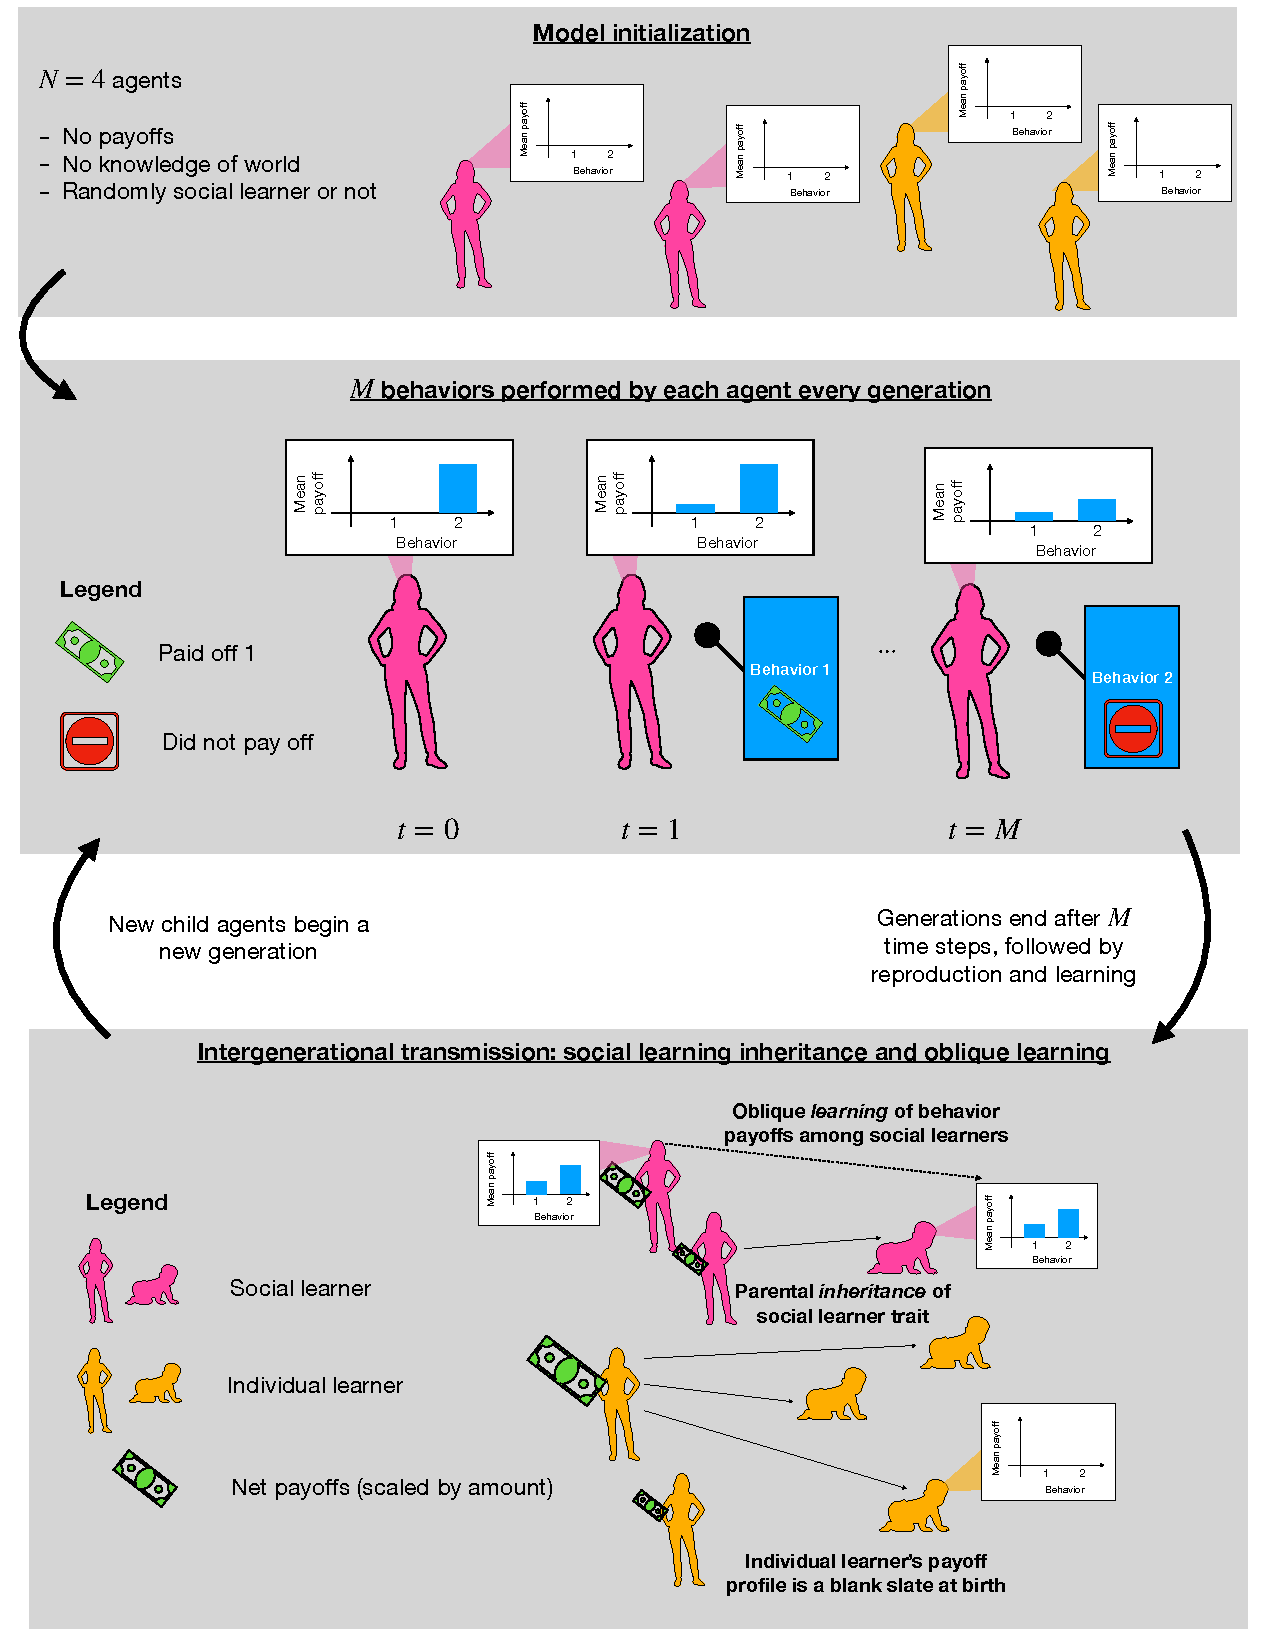
\includegraphics[width=0.9\textwidth]{Figures/IntraInterGenerationalDynamics.pdf}
  \label{fig:IntraInterGenerationalDynamics}
\end{figure}


\subsubsection{Initialization}

Model initialization includes agent and environment initializations. Agents are
randomly initialized to have the social learning trait or not, with equal 
probability. Agent ``ledgers'' and behavior counts 
are uniformly initialized to the no-knowledge,
blank-slate case where all $\pi_{ib} = 0$ and $c_{ib} = 0$. Both the 
ledger and behavior count vectors have $B$ entries, one for each
behavior the environment affords. Net payoffs for
the generation are also initialized to zero. All agents are initialized with
the same softmax temperature, $\tau$, that guides their behavior selection 
to be either more exploratory (greater $\tau$) or more exploitative of
what agents believe to be the optimal behavior(s) (lesser $\tau$).

The environment is initialized to have $B$ behaviors with one of them selected
at random to be the optimal behavior, denoted $b^*$. Behavior $b^*$ is 
initialized to have a probability $\pihigh$ of paying off 1. All other behaviors
are initialized to have probability $\pilow$ of paying off 1. The modeler must
specify the environmental variability, $u$, and the number of time steps per 
generation, $M$. 


\vspace{2em}
\begin{table}[h]
    \caption{Global environmental and cognitive initialization parameters.}
    \label{tab:modelParameters}
    \centering \hspace{-3em}
    \begin{tabular}{cp{4.0in}l} \toprule

        Symbol & Description & Values tested (bold$=$default) \\ 

        \midrule  

        $B$       & Number of possible behaviors (represented by ``bandits'') 
                  & 2, 4, 10 \\

        $\pihigh$ & Probability that the unique optimal behavior pays off 1 
                & \textbf{0.9} \\

        $\pilow$ & Probability one of $B - 1$ non-optimal behaviors pays off 1 
                 & 0.1, 0.45, 0.8 \\ 

        $\tau$ & Softmax temp.; $\uparrow=$more exploration, $\downarrow=$more
                    exploitation 
               & 0.01, \textbf{0.1}, 1.0 \\
        
        $u$    & Probability optimal behavior changes between generations 
               & 0.0, 0.1, \ldots, 1.0 \\

        $M$    & Number of time steps per generation & 1, $B/2$, $B$, $2B$, $4B$ \\

        $N_T$    & Number of teachers to pool, from which best selected 
                 & \textbf{5} \mt{TODO: Test more for sensitivity analysis?} \\

            
               
        \bottomrule
        \end{tabular} 
\end{table}
\vspace{2em}


\subsubsection{Intra-generational behaviors and payoffs}

Each generation begins with agents initialized either by the $t=0$ initialization
outlined above, or initialized via inter-generational reproduction and learning,
described in detail below. Within generations, there is no social learning.
At each time step within a generation, agents select a behavior to perform
using the softmax algorithm, then update their ledgers $\bar\pi_{ib}$ and behavior
counts $c_{ib}$. If 
the chosen bandit pays off for an agent, its net payoff is incremented by one,
$\pi'_i \leftarrow \pi_i + 1$. This process continues for $M$ time steps, 
when reproduction, learning, and die-off occur, re-initializing the next 
generation for performing $M$ behaviors selected via this same process.

At each time step, 
agent $i$ chooses behavior $b$ at random, with each behavior
weighted by the softmax function applied to that behavior's observed mean payoff
relative to all mean payoffs in the ledger,
\begin{equation}
  \Pr(i \text{ chooses behavior } b) = \frac{\exp(\bar\pi_{ib}
  / \tau) }{ \sum_{b=1}^B \exp(\bar\pi_{ib} / \tau)}.
\end{equation}  
Softmax behavior selection is a
biologically plausible model of behavior~\cite{Schulz2019} 
that enables agents to explore
alternative behaviors sometimes and exploit the best observed behavior other times,
in accordance with Luce's choice axiom~\cite{Luce1959},.
The parameter $\tau$ specifies how frequently alternative behaviors are
explored versus how frequently the best observed behaviors are 
exploited. Greater $\tau$ means more frequent exploration, lesser $\tau$ means
more frequent exploitation. We set $\tau = 0.1$ for
all computational analyses presented in the main paper. We (WILL HAVE) performed
sensitivity analyses and found a weak dependence on $\tau$ that does not affect our
main conclusions.

When agent $i$ performs behavior $b$, $i$'s behavior count 
is incremented by 1, $c'_{ib} \leftarrow c_{ib} + 1$. Agent $i$'s ledger of mean 
payoffs are updated % from $\bar\pi_{ib}$ to $\bar\pi_{ib}'$
using exponential weighted averaging, 

\begin{equation}
  \bar\pi_{ib}' = \bar\pi_{ib} +
    \frac{\mathrm{Bandit_{b}(0, 1)} - \bar\pi_{ib}}{c_{ib}'},
\end{equation}
where 
$\mathrm{Bandit}_{b}(0, 1)$
is 0 or 1 depending on the result of the bandit draw for behavior $b$. 


\subsubsection{Inter-generational inheritance and social learning}

Every $M$ time steps, agents from the current generation reproduce, teach,
and die, while the next generation to perform the next $M$ time steps learns
from one teacher from the previous generation if they inherited the social 
learner trait. Inter-generational dynamics thus depend on 
two payoff-biased selection mechanisms: reproducer selection
and teacher selection. 

$N$ reproducers are sampled from the population with
replacement weighted by net payoffs, i.e., at each of $N$ draws for a parent,
\begin{equation}
  \Pr(\text{Agent $i$ chosen for reproduction}) = \frac{\pi_i}{\sum_{i=1}^N \pi_i}.
\end{equation}
\noindent
We sample with replacement to allow for more successful agents to have multiple
offspring. Child agents inherit their parents' social learning trait, so 
all social learner parents spawn social learner offspring, and parents lacking
the trait spawn offspring lacking the trait. 

Child agents with the social learning trait then must select and learn from a
teacher from their parent's generation, including possibly their parent.
Child agents give no preference to whether potential teachers are social 
learners. A child selects a teacher by first selecting a pool of $N_T = 5$ potential
teachers. Among this pool, each child selects the teacher with the greatest
net payoffs. In case of a tie the teacher is chosen at random from those with
the shared maximum net payoff. 

Social learner child agents each acquire their teacher's ledger, and all social
learner children behavior counts are reset to 1 to limit ledger values to be between
0 and 1. Child agents without the social learner trait have all ledger and behavior
count values re-initialized to 0. At this point the re-initialized child agents
engage in behavior selection and payoff accumulation described above. 


\subsection{Computational analyses}

We manipulated environmental uncertainty parameters described above, $u$,
$\pisub{low}$, $B$, and $M$, to examine their effects on our
main outcome measure, the prevalence of social learning $s$. For each parameter setting
in our analysis we calculated the average value of $s$ at the final time step
of $T=1000$ across 100 runs for each combination of uncertainty parameter values.

To analyze the effect of various forms of uncertainty on social learning 
prevalence in our Analysis, we initialized several model runs with
different uncertainty parameters $u$, $\pisub{\mathrm{low}}$, $B$,
and $M$. We varied $u \in \{0.0, 0.1, \ldots, 1.0\}$ for each combination of
the following parameters:
$\pisub{low} \in \{0.1, 0.5, 0.8\}$, $B \in \{2, 4, 10\}$, $M \in \{B/2, B, 2B\}$.

\subsubsection{Outcome variables}

Our primary outcome variable is the mean prevalence of the social learning
trait over $N=100$ agents over 1000 trials at the final time step of each trial,
denoted $\meansl$.
Typically at the final time step all agents either have the social learning
trait or do not (see Supplement for a presentation of time series collections
and histograms of outcomes for
a representative sampling of variables \mt{TODO}).

\begin{table}[h]
    \caption{Global environmental and cognitive initialization parameters.}
    \label{tab:modelParameters}
    \centering \hspace{-3em}
    \begin{tabular}{cp{4.0in}l} \toprule

        Symbol & Description & Values \\ 

        \midrule  

        $\meansl$ & Mean social learning prevalence over agents and trials
                  & $\in [0.0, 1.0]$ \\

        $p_{\text{opt}}$ & Fraction of population performing optimal behavior
                         & $\in [0.0, 1.0]$ \\

        \texttt{count}$(b_i)$ & Number of agents performing behavior $b$ 
                              & Behavior-count key-value pairs\\
        \bottomrule
    \end{tabular}
\end{table}


\section{Analysis}

% \begin{itemize}
%   \item 
%     To understand how different forms of uncertainty affect social learning evolution
%     we systematically varied environmental variables in our model and observed
%     corresponding changes in mean social learning prevalence, $\meansl$. We
%     confirmed that, in many cases, increased environmental variability $u$ 
%     suppresses social learning. However\ldots 


%   \item 
%     Our analysis confirmed existing theoretical predictions that social learning
%     is valuable only when environments are sufficiently stable, i.e., 
%     environmental variability $u$ is sufficiently small.
%     Because of the central role of $u$, it is set on the x-axis in
%     all analysis plots shown in Figure~\ref{fig:results}. 
%     The threshold over $u$ at which social learning begins to decline
%     varies depending on the value of other environmental parameters. 

%   \item 
%     However, more possible behaviors $B$ ($B=2,4,10$ for the first, second, and
%     third column respectively in Figure~\ref{fig:results}) can lead
%     social learning to be selected for even for large values of $u$, possibly
%     due to the low risk and potentially high reward of learning an accurate
%     tally of mean payoffs from the previous generation. 
%     Since there are many behaviors and
%     few observations, softmax weighting will not significantly 
%     favor a sub-optimal behavior. However, if one does learn an accurate tally
%     then one does have an increased chance of performing the best one.

%   \item 
%     $\pilow$ can alter selection selection pressure for or
%     against social learning, depending on the number of time steps per generation.
%     For instance, when $B=2$, increasing $\pilow$ (i.e. increased uncertainty
%     about which behavior is optimal) leads at first to less sharp sigmoid curve, 
%     where social learning is less prevalent with increased $\pilow$ when
%     $u < 0.5$ and social learning is more prevalent with increased $\pilow$
%     when $u > 0.5$. When $\pilow = 0.8$ noise and genetic drift dominate across
%     tested values of $B$, with possibly a slight inverse correlation 
%     in social learning as $u$ increases. When $B \in \{4,10\}$, increasing
%     $\pilow \in \{0.1, 0.5\}$ leads uniformly to increased $\meansl$ over 
%     $u$ in those settings.     

%   \item
%     If $M/B$ has an effect it is mostly to 
%     increase reliance on social learning due to social information being of 
%     higher quality since teachers would have had more learning opportunities
%     for larger $M$. (THERE ARE CASES WHERE THIS IS NOT THE CASE BUT THERE IS 
%     STILL TOO MUCH NOISE DUE TO SMALL NTRIALS)

%   \item
%     Synthesis/analysis conclusion 
    
% \end{itemize}


\documentclass[varwidth=true,crop=false]{standalone}
\usepackage[chatter]{rotating}
\usepackage{amssymb,amsmath}
\usepackage{pgfplots}

\usepackage{geometry}
\geometry{
paperwidth=12in,
paperheight=12in,
margin=0.25in
}

\newcommand{\pisub}[1]{\pi_{\mathrm{#1}}}
\newcommand{\pilow}{\pisub{low}}
\newcommand{\pihigh}{\pisub{high}}
\newcommand{\piI}{\langle \pisub{I} \rangle}
\newcommand{\piS}{\langle \pisub{S} \rangle}
\newcommand{\ledger}{\bar\pi_{ib}}

\newcommand{\meanvar}[1]{\langle #1 \rangle}
\newcommand{\meansl}{\meanvar{s}}
\newcommand{\meanpi}{\meanvar{\pi}}
\newcommand{\meansoc}{\meanvar{\pi_\mathrm{S}}}
\newcommand{\meanasoc}{\meanvar{\pi_\mathrm{A}}}
\newcommand{\meanT}{\meanvar{T}}

\newcommand{\bandit}{\text{Bandit}_b(0, 1)}

\begin{document}
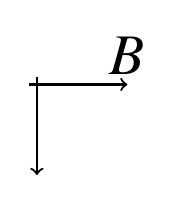
\begin{tikzpicture}
      \draw[->,thick] (-.1,0)--(1.15,0) node[above]
        {\huge $B$};
        % {Number of behaviors $B$};
      \draw[->,thick] (0,.1)--(0,-1.15) node[below]
        {\huge $\pilow$};
        % {Low payoff frequency $\pilow$};
	  \end{tikzpicture}~\\[-2em]

    \begin{minipage}{3.75in}
      \centering
      {\hspace{5.25em}\huge $B = 2$}
    \end{minipage}%
    \begin{minipage}{3.75in}
      \centering
      {\hspace{1.0em}\huge $B = 4$}
    \end{minipage}%
    \begin{minipage}{3.75in}
      \centering
      {\hspace{2.0em}\huge $B = 10$}
    \end{minipage}~\\

    \begin{minipage}{3.75in}
    \begin{rotate}{90}
      {\parbox{2.5in}{
          \centering
          \vspace{-2.5em} {\huge$ \pilow = 0.1$} \\
          {\begin{rotate}{-90}{\huge $\meansl$}\hspace{3em}\end{rotate}}
      }}
    \end{rotate}%
    \hspace{2em}
      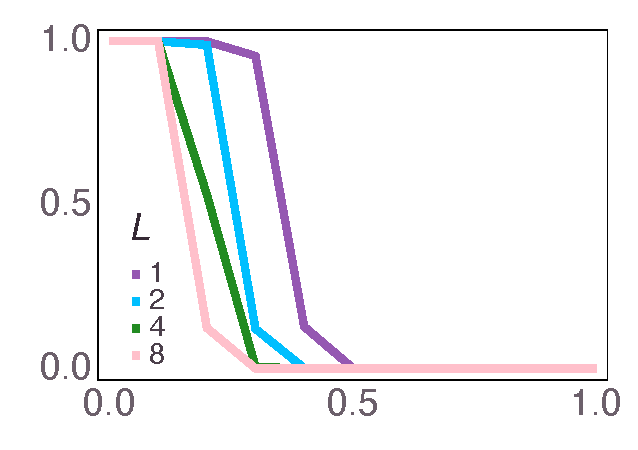
\includegraphics[width=\textwidth]{mean_social_learner_over_u_lowpayoff=0.1_nbehaviors=2.pdf}
    \end{minipage}\noindent\hspace{1.25em}
	\begin{minipage}{3.75in}%
      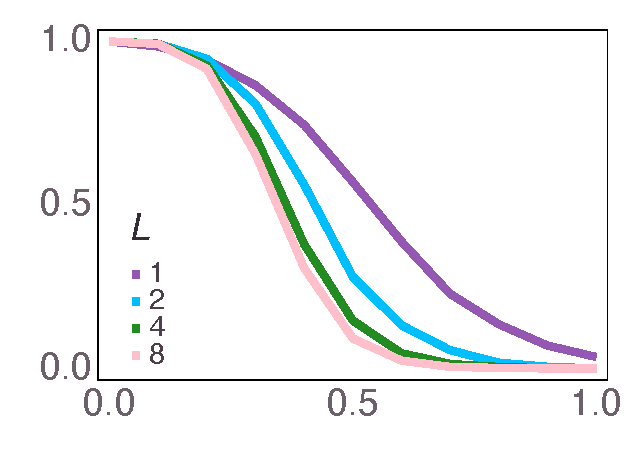
\includegraphics[width=\textwidth]{mean_social_learner_over_u_lowpayoff=0.1_nbehaviors=4.pdf}
    \end{minipage}\noindent
	\begin{minipage}{3.75in}%
      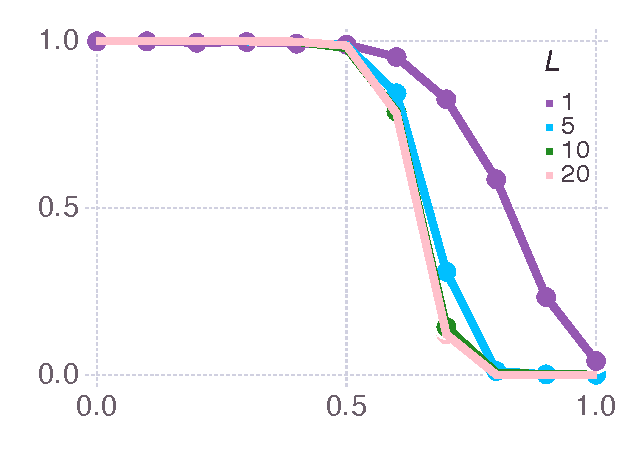
\includegraphics[width=\textwidth]{mean_social_learner_over_u_lowpayoff=0.1_nbehaviors=10.pdf}
    \end{minipage}~\\[0.5em]

    \begin{minipage}{3.75in}
    \begin{rotate}{90}
      {\parbox{2.5in}{
          \centering
          \vspace{-2.5em} {\huge$ \pilow = 0.45$} \\
          {\begin{rotate}{-90}{\huge $\meansl$}\hspace{3em}\end{rotate}}
      }}
    \end{rotate}%
    \hspace{2em}
      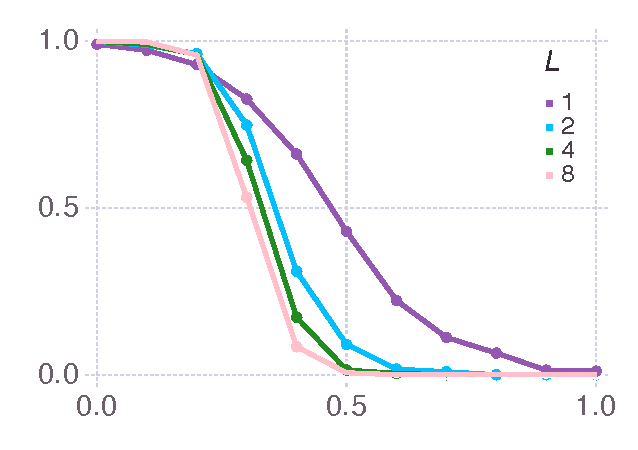
\includegraphics[width=\textwidth]{mean_social_learner_over_u_lowpayoff=0.45_nbehaviors=2.pdf}
	\end{minipage}\noindent\hspace{1.25em}
	\begin{minipage}{3.75in}%
      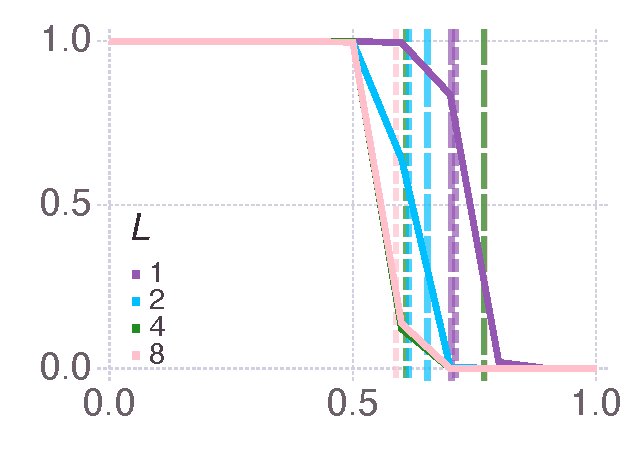
\includegraphics[width=\textwidth]{mean_social_learner_over_u_lowpayoff=0.45_nbehaviors=4.pdf}
    \end{minipage}\noindent
	\begin{minipage}{3.75in}%
      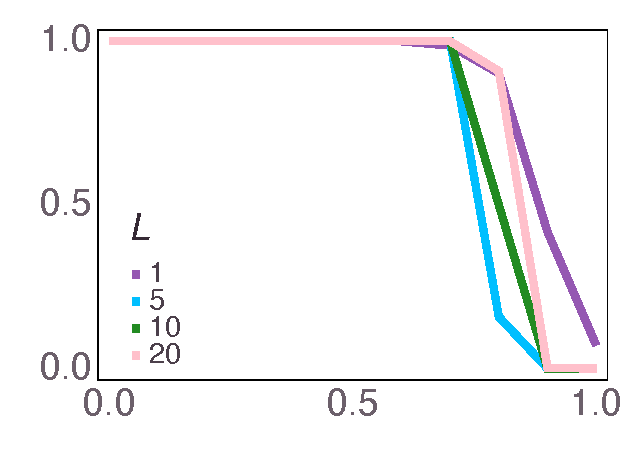
\includegraphics[width=\textwidth]{mean_social_learner_over_u_lowpayoff=0.45_nbehaviors=10.pdf}
    \end{minipage}~\\[0.5em]

    \begin{minipage}{3.75in}
    \begin{rotate}{90}
      {\parbox{2.5in}{
          \centering
          \vspace{-2.5em} {\huge$ \pilow = 0.8$} \\
          {\begin{rotate}{-90}{\huge $\meansl$}\hspace{3em}\end{rotate}}
      }}
    \end{rotate}%
    \hspace{2em}
      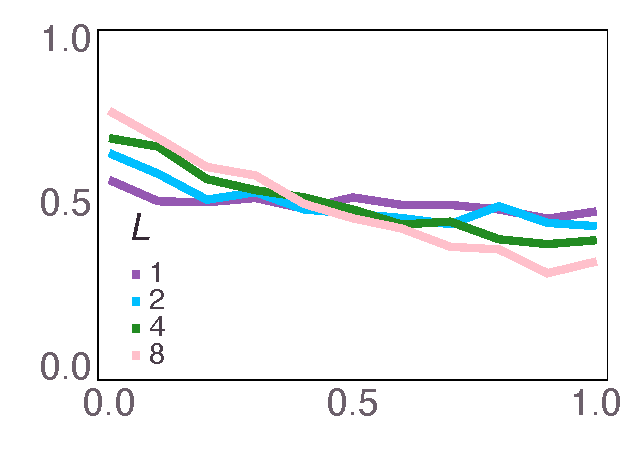
\includegraphics[width=\textwidth]{mean_social_learner_over_u_lowpayoff=0.8_nbehaviors=2.pdf}
        \\[-2.75em]
        \begin{center}
          {\hspace{3.25em} \huge $\quad u$}
      \end{center}
	  \end{minipage}\noindent\hspace{1.25em}
		\begin{minipage}{3.75in}%
		  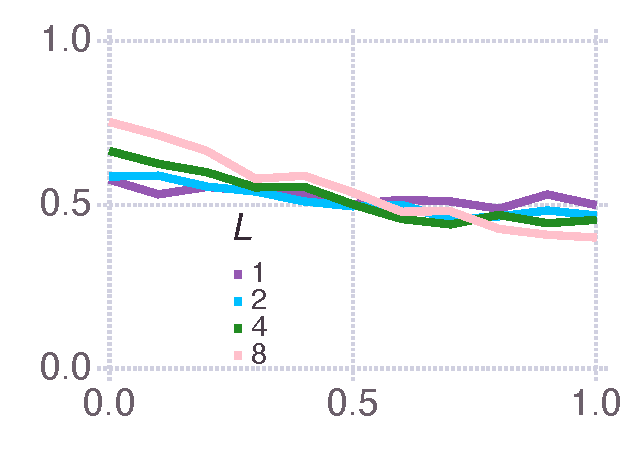
\includegraphics[width=\textwidth]{mean_social_learner_over_u_lowpayoff=0.8_nbehaviors=4.pdf}
		  \\[-2.75em]
	  \begin{center}
        {\huge $\quad u$}
      \end{center}
    \end{minipage}
	\begin{minipage}{3.75in}%
		  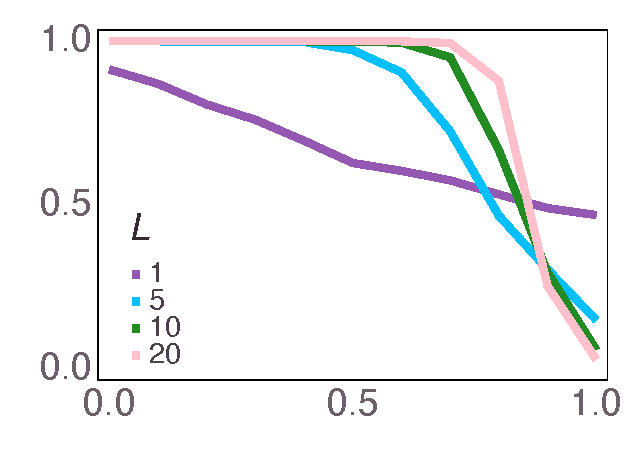
\includegraphics[width=\textwidth]{mean_social_learner_over_u_lowpayoff=0.8_nbehaviors=10.pdf}
		  \\[-2.75em]
	  \begin{center}
        {\huge $\quad u$}
      \end{center}
	\end{minipage}%
\end{document}


\section{Discussion}


\bibliographystyle{apacite}

\setlength{\bibleftmargin}{.125in}
\setlength{\bibindent}{-\bibleftmargin}

% \bibliography{/Users/mt/workspace/Writing/library.bib}
\bibliography{this.bib}

\end{document}
